\newpage
\section{Appendix}\label{chap:appendix}

\subsection{Measurement data for a coaxial RF line with various terminations}
The following table~\ref{tab:power_plots_1} shows the measured signal power along the coaxial line for loads: open, short and 100$\Omega$.
\begin{table}[ht!]
	\centering
	\begin{tabular}{|c||c|c|c|}
		\hline
	    \textbf{Adjusted} & \multicolumn{3}{c|}{\textbf{Measured}} \\
		\hline
		$d$ / cm &
		$P_{\mathrm{open}}$ / dBm &
		$P_{100\Omega}$ / dBm &
		$P_{\mathrm{short}}$ / dBm \\
		\hline\hline
		35.0 & -21.9 & -22.8 & -23.3 \\
		40.0 & -18.8 & -21.5 & -30.2 \\
		41.9 & -17.9 & -21.0 & -38.6 \\
		44.0 & -17.3 & -20.8 & -64.0 \\
		45.0 & -17.4 & -20.9 & -41.3 \\
		50.0 & -17.0 & -20.8 & -26.4 \\
		55.0 & -17.6 & -21.5 & -21.1 \\
		60.0 & -19.0 & -22.9 & -19.7 \\
		65.0 & -22.0 & -24.8 & -18.7 \\
		70.0 & -27.9 & -26.5 & -18.8 \\
		72.5 & -34.0 & -27.0 & -19.1 \\
		74.7 & -73.0 & -26.6 & -19.6 \\

		80.0 & -26.8 & -24.9 & -21.8 \\
		85.0 & -21.5 & -23.0 & -25.9 \\
		90.0 & -19.0 & -21.9 & -35.9 \\
		92.3 & -18.0 & -21.5 & -63.5 \\
		95.0 & -17.7 & -21.3 & -34.0 \\
		100.0 & -17.5 & -21.4 & -25.0 \\
		105.0 & -18.2 & -22.2 & -21.3 \\
		110.0 & -20.2 & -23.8 & -19.5 \\
		115.0 & -23.7 & -25.7 & -18.9 \\
		120.0 & -31.0 & -27.0 & -19.1 \\
		123.0 & -71.0 & -26.7 & -19.6 \\
		125.0 & -35.5 & -26.0 & -20.3 \\
		130.0 & -24.5 & -24.1 & -22.7 \\
		135.0 & -20.7 & -22.3 & -27.9 \\
		136.6 & -19.0 & -21.8 & -31.9 \\
		138.5 & -18.3 & -21.5 & -38.6 \\
		140.0 & -18.1 & -21.3 & -48.0 \\
		140.5 & -19.8 & -21.1 & -63.5 \\
		145.0 & -17.1 & -20.9 & -29.4 \\
		150.0 & -17.2 & -21.2 & -23.0 \\
		155.0 & -18.0 & -22.1 & -20.1 \\
		160.0 & -20.0 & -23.7 & -18.5 \\
		165.0 & -24.5 & -25.4 & -18.0 \\
		\hline
	\end{tabular}
	\caption{\centering Measured gain values versus distance for the first set of terminations.}
	\label{tab:power_plots_1}
\end{table}

\FloatBarrier
\newpage
The following table~\ref{tab:power_plots_2} shows the measured signal power along the coaxial RF line for the loads: capacitive load, 25$\Omega$ and 50$\Omega$.
% Table generated by Excel2LaTeX from sheet 'Tabelle2'

\begin{table}[ht!]
\centering
\begin{tabular}{|c||c||c|}
    \hline
    \textbf{Adjusted} &
    \textbf{Measured} &
    \textbf{Datasheet} \\
    \hline
    $f$ / Hz & $e_n$ / nV$/\sqrt{\mathrm{Hz}}$ & $e_n$ / nV$/\sqrt{\mathrm{Hz}}$ \\
    \hline\hline
    10 & 6.810 & 6.4 \cite{Amp} \\
    1.0k & 2.752 & 2.7 \cite{Amp} \\
    \hline
    \end{tabular}
    \caption{\centering Values corresponding to the OpAmp noise model check at 10\,Hz and 1.0\,kHz (Gain = +1).}
    \label{tab:sim_2}
\end{table}


\newpage
\subsection{Resultant plots from measurement data}
The following figure~\ref{fig:chart3} shows the resultant plot of the measured signal power values, for all 6 termination loads in the same chart, along the coaxial transmission line.
\begin{figure}[ht!]
	\centering
	\includegraphics[page=4,width=0.9\linewidth]{src/diagrams/RF_1/Chart_3}
	\caption{\centering Measured power values for every termination load.}
	\label{fig:chart3}
\end{figure}

\subsection{Code snippets used for calculations}

The following code \ref{lst:load-code} is used to compute the Load impedance.
\lstdefinestyle{mystyle}{
	basicstyle=\ttfamily\small,
	breaklines=true,
	columns=fullflexible
}

\begin{lstlisting}[style=mystyle, language=Python, label={lst:load-code}]
import cmath
import math

Z0 = 50  # characteristic impedance in ohms
mag = float(input("Enter reflection coefficient magnitude |Gamma|: "))
phase_deg = float(input("Enter reflection coefficient phase in degrees: "))

phase_rad = math.radians(phase_deg)
Gamma = mag * cmath.exp(1j * phase_rad)
ZL = Z0 * (1 + Gamma) / (1 - Gamma)

print(f"\nGamma = {Gamma.real:.6f} + j{Gamma.imag:.6f}")
print(f"Load impedance ZL = {ZL.real:.6f} + j{ZL.imag:.6f} ohms")
\end{lstlisting}

\newpage
The following code \ref{lst:load-code} is used to represent the reflection coefficient on the smith chart.
\begin{lstlisting}[style=mystyle, language=Python, label={lst:smith-code}]
	import matplotlib.pyplot as plt
	import pysmithchart
	
	Z0 = 50
	Z = [
	1e9 + 0j,   # Open
	0 + 0j,     # Short
	100 + 0j,   # 100 ohm
	25 + 0j,    # 25 ohm
	50 + 0j,    # 50 ohm
	0 - 50j     # Capacitive load
	]
	labels = ["Open", "Short", "100Ω", "25Ω", "50Ω", "Capacitive"]
	colors = ["red", "blue", "green", "orange", "purple", "brown"]
	
	plt.figure(figsize=(9, 9))
	ax = plt.subplot(111, projection="smith", Z0=Z0)
	
	for z, label, color in zip(Z, labels, colors):
		ax.plot([z], marker="o", markersize=10, color=color, ls="")
		ax.text(z, label, color=color)
		
		ax.set_title("Smith Chart of 6 Load Impedances")
		plt.tight_layout()
		plt.show()
\end{lstlisting}

\newpage
